\PassOptionsToPackage{svgnames,x11names}{xcolor}
\documentclass[10pt,conference]{IEEEtran}
\usepackage{todonotes}
\usepackage{listings}
\usepackage{multirow}
\usepackage{float}
\usepackage{placeins}
\lstset{language=prolog, breaklines=true, basicstyle=\small, escapeinside={(*}{*)},
	moredelim=**[is][\color{green}]{|+}{|},
	moredelim=**[is][\color{red}]{|-}{|}
	}

\usepackage[draft]{djb}
\usepackage{shortcuts}

\begin{document}

\newcommand{\subheading}[1]{\textbf{#1.}}

\title{Detecting Use-after-Free through Alias Analysis in Compiled Code}
\author{Matthew Maurer}
\maketitle
\begin{abstract}
	%Scope Statement
%tl;dr I want to deal with the interaction of binary analyses
This thesis is focused on the interleaving, interaction, and scheduling of analyses over binary code.
%Compiled code, sans source, is everywhere
Most commercial software tends to come in the form of a compiled binary sans source.
%Compiled code needs to be analyzable
This software needs to be analyzable in order to allow for security audits of libraries and executables, continued use of legacy code, and attack development.
%This is difficult because binaries are turing complete, and even "well behaved" code does crazy shit
Analysis of compiled code provides a number of unique challenges due to the stripping away of information the original programmer had access to, such as intended control flow information, types, and variable locations.
%General statement about how we can help?
A wide variety of techniques for attacking this problem from different angles have been developed, but are typically resource intensive and not integrated with one another.

%Previous Work
%VSA
%Jakstab
%Types shit
Previous work in analyzing binary code has performed type recovery\cite{bitr}, variable identification\cite{divine}, control flow recovery\cite{jakstab,phoenix}, and value analysis\cite{vsa}.
However, this work tends to have issues with the relative expense of running the analyses, the coupling between analyses, and the integration of the current state of the art in each area.
While many interesting analyses have been developed, cooperation and integration of these analyses has been largely ignored.

%This is Holmes
I intend to build \sysname, a logic language inspired by Datalog with several features geared towards the ability to use a logic program as a means of coordinating several independent analyses.
%Features:
% Forwards + Backwards chaining
% Caching
% Remote user defined predicates
% Scheduling
% Combining
By providing the ability to expose external functions to the language, and allowing them to transform bound variables during rule execution, \sysname\ will allow the use of other paradigms and languages for writing analyses.
Binding analyses to rule firing also allows the framework to provide caching, re-running analyses only when needed.
\sysname\ will mix forwards and backwards chaining execution, defined per rule, to enable the rapid processing of things that will nearly always want to be done, such as lifting of reachable addresses to an intermediate language, while allowing for goal-directed execution of longer procedures such as fuzzing campaigns.
These per-rule planning hints form the beginning of scheduling rules which are costly or non-terminating.
\sysname\ will provide a mechanism for registering combining functions for related facts to a subsuming fact for simpler reasoning about accumulated information.
The logic language representation of knowledge provides a good way to deal with the partial information that tends to be imparted by program analyses. As more new facts are generated, the dependencies in the rules make it explicit which rules can use the new information.

%Work Plan
\sysname\ provides a way to mesh the many existing styles of analysis together, taking into account the potential for nontermination or high cost of various analyses. This thesis will provide semantics for the \sysname\ language, an implementation of a program which actually runs the language, and example applications coordinating multiple analyses to achieve better results than they could achieve alone.

\end{abstract}
\section{Introduction}
In order to show that Holmes can be used in practice, we implement a concrete system with it.
We chose to focus on the problem of use-after-free, as it is a little-explored area for static binary analysis.
We used Holmes here to link together control flow analysis, alias analysis, string recovery, and general function loading in order to build a working use-after-free engine.

% Use after free bugs are common
There were 238 use-after-free (UaF) vulnerability disclosures (CWE-416) issued in 2017 alone, with 36.2\% given a critical security
rating.
% From cvedetails.com, mitre doesn't seem to issue CVE/CWE associations.
Use-after-free bugs happen when a pointer has been freed and the memory pointed to subsequently written to or read from.
Use-after-free bugs can lead to DoS, control flow hijack, and information leaks.

Despite the number of CVEs, few tools exist that can automatically and statically detect such bugs in off-the-shelf \emph{binary} code.
However, there are tools for finding such bugs in \emph{source} code.
Requiring source code limits the applicability of these techniques to developers with full source access.

In this chapter, we focus on the question
``Can we use \sysname\ to bridge the gap between analysis for UaF bugs in source code versus compiled code?''
In particular, previous work has been unable to apply source code techniques to compiled code.
Can we adapt such techniques to be effective even without source?

At a high level, UaF bugs require reasoning about memory allocation and memory aliasing.
Source code techniques are more plentiful due to the rich and mature research area of alias, points-to, and similar schemes for reasoning about memory over the lifetime of a program.
In comparison, at the binary level the primary approach for reasoning about memory is Value Set Analysis~\cite{vsa}, which is less mature and has several limitations in practice such as inability to reason about all arithmetic operations (e.g., bit-shifts and division) and the fact it may not terminate without ad-hoc widening in the presence of loops.
For example, GUEB~\cite{gueb} was proposed to detect UaF bugs using VSA, but is handicapped by disallowing cyclic paths to allow rapid termination of VSA.

We present a new binary-level static analysis approach for detecting UaF bugs in executable programs.
One of the main technical challenges we address is showing how to adapt source-code memory alias analysis to compiled code, where previous work has instead created all-new binary-only approaches to alias
analysis like VSA.
We experiment with two classes of analysis: flow insensitive alias analysis via a Steensgaard-type~\cite{steensgaard-alias} algorithm, and  flow-sensitive alias analysis using a data flow approach adapted from Andersen~\cite{andersen} style analysis with added rules to handle binary-specific details such as calling conventions and computed addresses.
We also add context-sensitivity by allowing the analysis to reason about the call-stack discipline followed by executable code, and a type of field sensitivity appropriate for direct pointer arithmetic without type information.
To the best of our knowledge, very little work has been done in applying the literature in source alias analysis to compiled code, and no previous work has shown how to then use such techniques to find UaF bugs statically in compiled code.

We have built a tool called \aliasname\ that uses \sysname\ to drive the different levels and co-dependencies in binary analysis, alias analysis, and UaF detection.
Taking this approach allows us to have an end-to-end reasoning chain from input binary to why this particular candidate use-after-free could not be disproven with a given sensitivity.

We evaluated \aliasname\ over 7 real CVEs and the Juliet test suite released by IARPA for purposes of verifying our detection capabilities and measuring false positives in the face of bugs.
Additionally, we measured false positive rates against a background of expected-good binaries (we assume no true positives): a random sampling from the \texttt{\$PATH} of a default Ubuntu installation.

\aliasname\ is available at \url{https://github.com/maurer/marduk}.

\section{Background}
\subsection{Alias Analysis}
An alias analysis endeavors to answer the question ``Do these two pointers point to the same thing?''
There are two basic varieties: may and must alias.
Must alias means that two values will definitely point to the same thing, but the lack of such a relationship means nothing.
May alias means that two values might point to the same thing, and the lack of such a relationship means they definitely will not.

Additionally, alias analyses have different degrees of sensitivity.
The sensitivity of an alias analysis refers to what additional parameters the analysis examines when asking whether two pointers alias.
A flow-sensitive analysis uses the program counter or statement location as a parameter.\footnote{
This implicitly encodes the location within the control flow graph since the analysis is also conditioned on the particular compilation of the source program.}
A context-sensitive analysis uses program call stack as a parameter.
This term is also sometimes used to discuss the granularity of the memory model in use, e.g. a ``field sensitive analysis'' is one in which the model distinguishes between writes to \texttt{s->x} vs \texttt{s->y}.
In our case, a lack of type information and the presence of pointer arithmetic adds complexity to field sensitivity, so it differs from the traditional presentation (\S~\ref{sec:field}).

Analysis which is both context and flow insensitive is generally efficient, in nearly linear time~\cite{steensgaard-alias}.
However, their lack of sensitivity makes the drawing of variable boundaries important and removes all ability to reason about a variable being overwritten as a safety property.
Common examples of this are Steensgaard~\cite{steensgaard-alias} and Andersen's~\cite{andersen-alias}.

Flow-sensitive analyses are still more seldom used due to their longer run times, but modern techniques are beginning to allow them to scale to larger codebases~\cite{sfs}.
Flow sensitivity is the most important sensitivity for our use case because it helps us to reason about overwritten variables.
For example, if the program frees a variable, then overwrites it with a fresh pointer (for example, \texttt{free} followed by \texttt{strdup}), this avoids leaving the variable as potentially free.
It is additionally specifically important to the binary domain due to the repeated re-use of registers.
Over the course of a function, the register \texttt{RAX} probably maps to multiple different variables, depending on the current program counter.
Flow sensitivity helps to keep these relationships separated by parameterizing the alias relationship accordingly.
The implementation of a flow sensitive analysis generally follows the pattern of performing dataflow on a points-to relationship to a fixpoint.

Context-sensitive analyses are frequently used in analysis of Java and other object oriented programs because it helps to reason about which class of objects may have been the argument to a function, and thus which methods may be the target of the call.
The two primary ways to accomplish this are to either take a call-site approach (tracking a stack of return addresses), or an object based approach where method calls take as a parameter which objects they may have occurred on.
We will focus on the call-site approach in this thesis as not all the code under examination is object oriented, and we are not performing object recovery on the code which is.

The call-site approaches are generally distinguished from one another based on the domain used for the stack tracking.
With an unbounded stack, it reduces to inlining every function call.
This can result in an expansion of problem size, and cannot terminate in the case of recursion.
If an analysis can handle the larger control flow graph, it can special case out recursion by either contracting strongly connected components of the function call graphs to single nodes, or by truncating stacks on recursive calls to the last time this call site occurred.
Another option is to limit how much of the context the domain tracks.
A common approach is to limit the domain by tracking only the most recent $k$ calls for some fixed $k$.
In this case, a strategy to deal with recursion is not required, but may still prove useful to put available precision to the best use possible.

One of the most focused on analyses for alias analysis over binaries is VSA~\cite{vsa}.
VSA integrates the problem of alias and value analysis by doing abstract interpretation over a domain called a strided interval, with dynamic allocations appearing as free variables.
This formulation has produced useful results in the past, but its relative expense~\cite{angr-sok} has limited its applications, especially with regards to whole program analysis.
The authors of VSA also applied to variable recovery~\cite{divine}.


\section{Previous Approaches and Related Work}
%Related Work
\section{Related Work}
\label{sec:related}
%  Starting blurb similar to backround blurb, surprised by this...
As this work stands at the confluence of compilation, instruction set architectures, static analysis, and type theory, there is a great deal of prior work that provided the foundation to create \bitr. There have been other attempts to perform binary type recovery. Type theorists have explored the relevant formal systems that enable us to appropriately describe the constraints imposed by the wide variety of instructions. Others have tried to build decompilers, each of which contains at least an attempt at type reconstruction.
%  Chunk related work into blobs and describe, reference to sections as you do it
\subsection{Types in Compiled Code}
In large part, previous work has considered dynamic approaches, which use execution traces to get information about concrete values. Another school of thought takes a more forensics-oriented approach, attacking the problem by looking for known data structures within a dump or trace. Finally, there is the school to which this work belongs, static type recovery, where the approach regenerates type information from a representation of the code, rather than from sample runs or matching known data structures.

\noindent {\bf Dynamic Type Description.}
Rewards~\cite{rewards} takes a dynamic, trace-oriented approach to the problem, taking execution traces and known system calls, and propagating types from system calls through the trace's reads and writes. The dynamic approach has the advantage that the analysis can know what values a memory location or register actually held at a given program point. Additionally, the dynamic approach does not have to solve the problem of indirect jumps, as when working with traces the next instruction is precisely computed. Finally, since Rewards had exact aliasing information via pointer values on each trace, flowing information from the system call barrier (their major outside source of types) is easier. While Rewards seems limited for types not present during the crossing of the system call barrier, its dynamic approach, and information from the crossing of the system call barrier could provide additional constraints to a system like \bitr\ to further improve accuracy. Howard~\cite{Slowinska2011} extends the work of Rewards by focusing on access patterns instead of simple propagation, and annotating variables from the original code, rather than locations on a dump.

\noindent {\bf Type Forensics.}
Another approach known as shape analysis~\cite{August, Haller2013a,White2013,Jung2009,Cozzie} uses dynamic traces to generate shape graphs, which they then analyze to make guesses at the types of memory locations. The systems generate the shape graph by first generating a trace, then matching the access pattern to the simplest possible graph of type structures. Some generate this trace from the compiled program, and some must annotate the program prior to compilation to achieve this trace. Once the system generates the shape graph, it compares the shape graph to multiple possibilities of what the data structure might be in attempt to classify it e.g. as a binary tree or linked list. One benefit of this technique is that when the system finds a match, more information on a name of the data structure may be available. However, if the program uses a data structure not expected by the system, some of these methods will fall short. For example, MemPick will report it to be a generic graph. It also suffers from the standard dynamic analysis issue of being unable to generate types for paths the test cases did not drive it down.

\noindent {\bf Static Type Recovery.}
Like TIE~\cite{tie}, we built \bitr\ on BAP~\cite{bap}, and also took the approach of trying to generate ranges of constraints. However, TIE performs much worse under our metric, which we feel more fully represents accuracy of more complicated types. TIE's metric is problematic for the reasons described in~\cite{sw}, but the proposed replacement metric is still dependent on a notion of distance. TIE is also slow, which hobbles its use as a large scale analysis tool. The use of DIVINE's methods was one of the bottlenecks, which we avoided in \bitr\ by recovering the type of everything that is addressable through the registers or a constant integer used along a dataflow that ended in a read or write. While the type system of TIE included structure types, TIE would rarely infer them, though its metric did not demonstrate this. Finally, if run on a static binary (e.g. without dynamic library hints), the amount TIE could infer itself was minimal.

SecondWrite~\cite{sw} instead takes the approach of lifting to a LLVM-based IR~\cite{llvm}, then using \texttt{mem2reg} to detect variables and LLVM pointer analysis to compute the types. Their reconstruction is simpler and faster than TIE's, but the approach has issues: \texttt{mem2reg} is a nice shortcut, but has the problem that \texttt{mem2reg} will not promote anything which has a use other than a load or store~\cite{llvm}. As a result, if on-stack references are in use, those stack slots will not be properly promoted to variables. Additionally, dependence on pointer analysis leaves them without a way to detect recursive types within their framework, and makes nested structures unlikely to work.

Another work focusing primarily on structure recovery~\cite{comprecon} approached the problem from the angle of figuring out what idioms compilers used to address arrays and structs, and then tried to reconstruct structs and arrays. However, by the authors' own admission, this approach cannot handle nested structs. Additionally, their dependence on assumptions about how the compiler will act and how the source language must work cause the output to be of limited use for understanding properties of code which was not necessarily built by the compilers or language expected.

\subsection{Type Theory}
Some of the inspiration for this form of type characterization \S\ref{sec:typesys} came from intersection typing~\cite{Jim1995,Shao1993}. Though we did not end up using intersection types for inferrability purposes (even the decidability of the inference turns out to be difficult and limited~\cite{interdecide}), this work informed our choice of a constraint-intersection \S\ref{sec:infmeth} approach instead of type-intersection approach.

Earlier efforts to generate typed assembly~\cite{tal,stal} also bear similarity to our work. Typed assembly language methodologies are attempting to assign types to the registers in compiled code during compilation. Some of the TAL ideas are applicable, and still others could potentially help in future reconstruction work as safer types.
However, the majority are inappropriate for the work because the compiler or author must make the code conform to the system, rather than the system describing the code.

\subsection{Decompilation}
One of the main applications for type reconstruction is decompilation. Some approaches~\cite{tydecomp} even suggest that the type reconstruction can help guide the decompilation itself rather than simply being a set of annotations applied at the end. This idea has existed~\cite{dolgova2009automatic} in decompilation for a while, but progress has been slow. More recent decompilers~\cite{phoenix} have used some of the other research~\cite{tie} in the area to improve their results as well. Given the poor state of affairs in Hex-Rays~\cite{ida}, more work in this field could improving the usability of much of the decompiler work would not be surprising.

\section{Alias Analysis Design}
\label{alias:sec:system}
First, our system transforms the input binary into structured
semantics we can work with throughout the rest of the process.
Second, we perform alias analysis over the structured representation.
This allows us to know all the pointers which may point to freed
memory after each free.  Finally, we look for reads and writes through
potentially freed pointers to create our list of candidate
use-after-frees.

\subsection{Alias Analysis}
Alias analysis consists of computing the possible ways to access different variables.
If dereferencing two expressions may access the same variable, they are said to alias.

Our machine-level alias analysis involves three main design choices that must be addressed:
\begin{enumerate}
\item Selecting variables.
  Alias analysis is performed over program variables, but unlike C, the assembly from a binary does not contain variable information.
\item Selecting sensitivity.
  We can return points-to information parameterized on different pieces of context.
  Common examples of parameters are flow sensitivity (program location), context sensitivity (call stack), field sensitivity (offsets within memory regions), and object sensitivity (possible construction sites for a ``this'' pointer).
  In this work, we examine, flow, context, field, and recency~\cite{vsa}, how to implement them on compiled code, and their effects on precision and performance.
\item Solving for points-to relationships.
  The generation of the aliasing information is undertaken differently for flow-insensitive vs flow-sensitive varieties of alias analysis.
  The flow-insensitive variety uses a constraint satisfaction technique and simultaneous solving via Steensgaard~\cite{steensgaard-alias}.
  Flow-sensitive varieties use the inter-procedural dataflow described in \S \ref{sec:interproc}.
\end{enumerate}

\begin{figure}
	\centering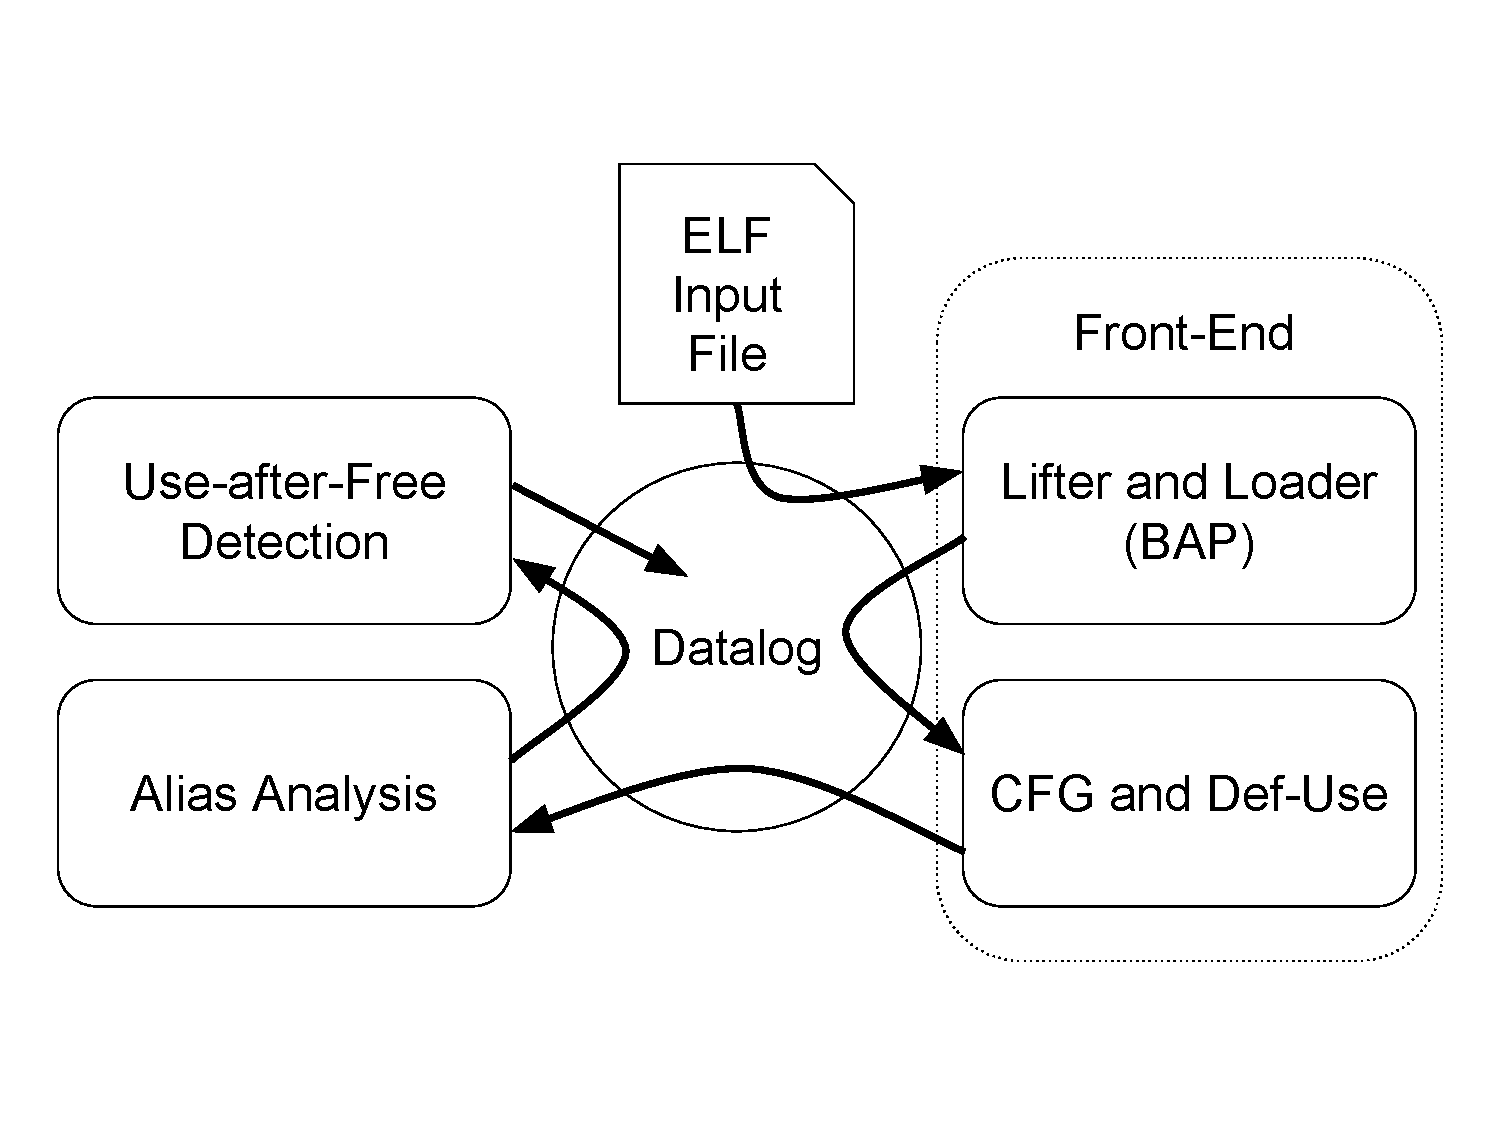
\includegraphics[scale=0.3]{alias/system.pdf}
	\caption{System Diagram}
	\label{fig:system}
\end{figure}

\subsection{Front-End}
Before we can apply our analysis, we first need to transform the raw
bytes of the input file into a form similar to the AST\footnote{Abstract Syntax Tree} received after
parsing.  Techniques in this section are not novel, and are described
for completeness to understand our overall system.

The front end:
\begin{itemize}
  \item Parses the executable file container, e.g., ELF on Linux
  \item Finds potential function entry points
%TODO if I do a codependence trial, forward reference here
  \item Builds a control flow graph
  \item Provides an intermediate language with the semantics for every reachable instruction
  \item Builds a call graph and call-site information
\end{itemize}

We use the BAP~\cite{bap} framework to provide ELF parsing, entry point identification, and instruction semantics.

\subheading{Variables}
In our approach, we use 3 kinds of variables:
\begin{itemize}
	\item Stack slots, parameterized by which function they are in. Written \texttt{sp+off@func}
	\item Registers
	\item Dynamic Allocations, parameterized by the location at which they are allocated. Written \texttt{dyn@loc}
\end{itemize}
We use an abstract location in these parameterizations.
In the context-insensitive case it is simply the address of the instruction, and in the context-sensitive case it is the pair of the address with the return stack.

Our choice of dynamic allocation variables defines our heap model.
We assume that two memory regions may only alias if they were allocated at the same program point.
This assumption matches reality unless a pointer has been released back to the allocator via free, but then used afterwards (a use-after-free bug).
This may violate the assumption because a write to or read from the now freed pointer may alias with newly returned memory.
As a result, this heap model is correct at least until the first use-after-free in an execution.
As we are not performing a value analysis, we also assume all accesses are in-bounds.
Essentially, if a use-after-free is the \emph{first} memory violation to occur, we will locate it.

\subheading{Calculating Update Summaries}
In order to avoid analyzing the full complexity of IL instructions within alias analysis, we first transform them to contain only the relevant dataflow information.
Our update summaries are then a description of the action of an IL instruction on the points-to relationship, where \texttt{a} and \texttt{b} are variables as defined above:

\begin{itemize}
\item \texttt{a = b}
\item \texttt{a = *b}
\item \texttt{a = \&b}
\item \texttt{*a = b}
\item \texttt{*a = *b}
\item \texttt{*a = \&b}
\end{itemize}

A list of these is generated for each instruction and associated with
the location of the instruction.  At allocation sites we emit the
summary \texttt{a = \&dyn@loc}, meaning that the variable \texttt{a}
(usually \texttt{RAX}) takes on the address of the allocation region
corresponding to that location.  % In our example~\ref{lst:example-asm}
% we would emit \texttt{RAX = \&dyn@0} for the instruction on line 4
% (location 0).  In the context-insensitive case, this gives us an
% abstraction parameterized only on the address of the malloc; values
% from one allocation site are assumed to never alias with those from
% another.  In the context-sensitive cases, this summary additionally
% parameterizes the abstraction by the return stack at allocation time.

\subsection{Insensitive Analysis}
In the flow-insensitive case, we modify the summaries before use to adapt our variable selection to better fit the problem.
Specifically, we annotate registers with definition sites, similar to what might be found in SSA form.

We compute the possible definition sites of each register on the right side of a summary, and clone the summary for every possible definition.
If the left side of a summary contains a register, we parameterize it with the location it came from.
We do this because a single register may hold many different logical variables at different points of time.
The register location parameterization allows us to avoid every definition of a register being potentially readable from every other site in the program.
Without our approach, the resulting alias sets would be too imprecise to be useful as a register's alias set (e.g., \texttt{RAX}) would include information about all variables ever assigned to \texttt{RAX} by register allocation.
Notably, this would include every call to \texttt{malloc}.
This parameterization adds a little bit of flow sensitivity even in otherwise insensitive analysis.

We then aggregate all update summaries from the program and solve them by equality via Steensgaard's algorithm.
Steensgaard runs  in almost linear time~\cite{steensgaard-alias} making it possible to compute over nearly any binary, though is less precise than flow-sensitive analysis, described below.
We use insensitive analysis as a baseline to help quantify the additional precision derived by adding additional sensitivity.




\subsection{Adding Flow Sensitivity}
Our flow sensitive analysis is structured as a dataflow problem.  At each assembly instruction, we use a transfer
function based on Andersen's~\cite{andersen} inclusion-style analysis.
We use the inter-procedural dataflow adaptation described next (\S\ref{sec:interproc}).
The same rules and functions are used to handle both context-sensitive
and context-insensitive analysis, as the Location's stack context is
considered optional.

A dataflow analysis is defined by a transfer function which calculates how a statement should update the dataflow facts
(alias sets in our case),
a set of control flow edges to walk from a set of starting points,
and a meet function with specifies how to merge information sets at control flow graph confluence points.
We describe these below.

By default, alias analysis calculates alias sets even when a variable is dead.
We run a pass before alias analysis to determine which variables are live.
While calculating alias analysis, we use this information to remove dead points-to information to improve performance and precision.
Performance is increased because we do not waste time and space updating and tracking points-to
sets we know will never be used.
Precision is increased because if no pointers to a given allocation exist any longer, we know any new pointer to that allocation points to copy of that region which does not need the information from the old copy.

\subheading{Transfer Function}
The actual processing of the update summaries based on summaries is calculated via the transfer function.
We follow Andersen as shown in Listing \ref{lst:process}:
\begin{itemize}
\item Definitions of variables are performed destructively.
\item Writes through variables are applied to each value they may point to.
\item Right hand sides go through 0, 1, or 2 levels of dereference for \texttt{\&b}, \texttt{b}, and \texttt{*b} respectively to generate the set to update with
\end{itemize}

\begin{figure}
	\centering
	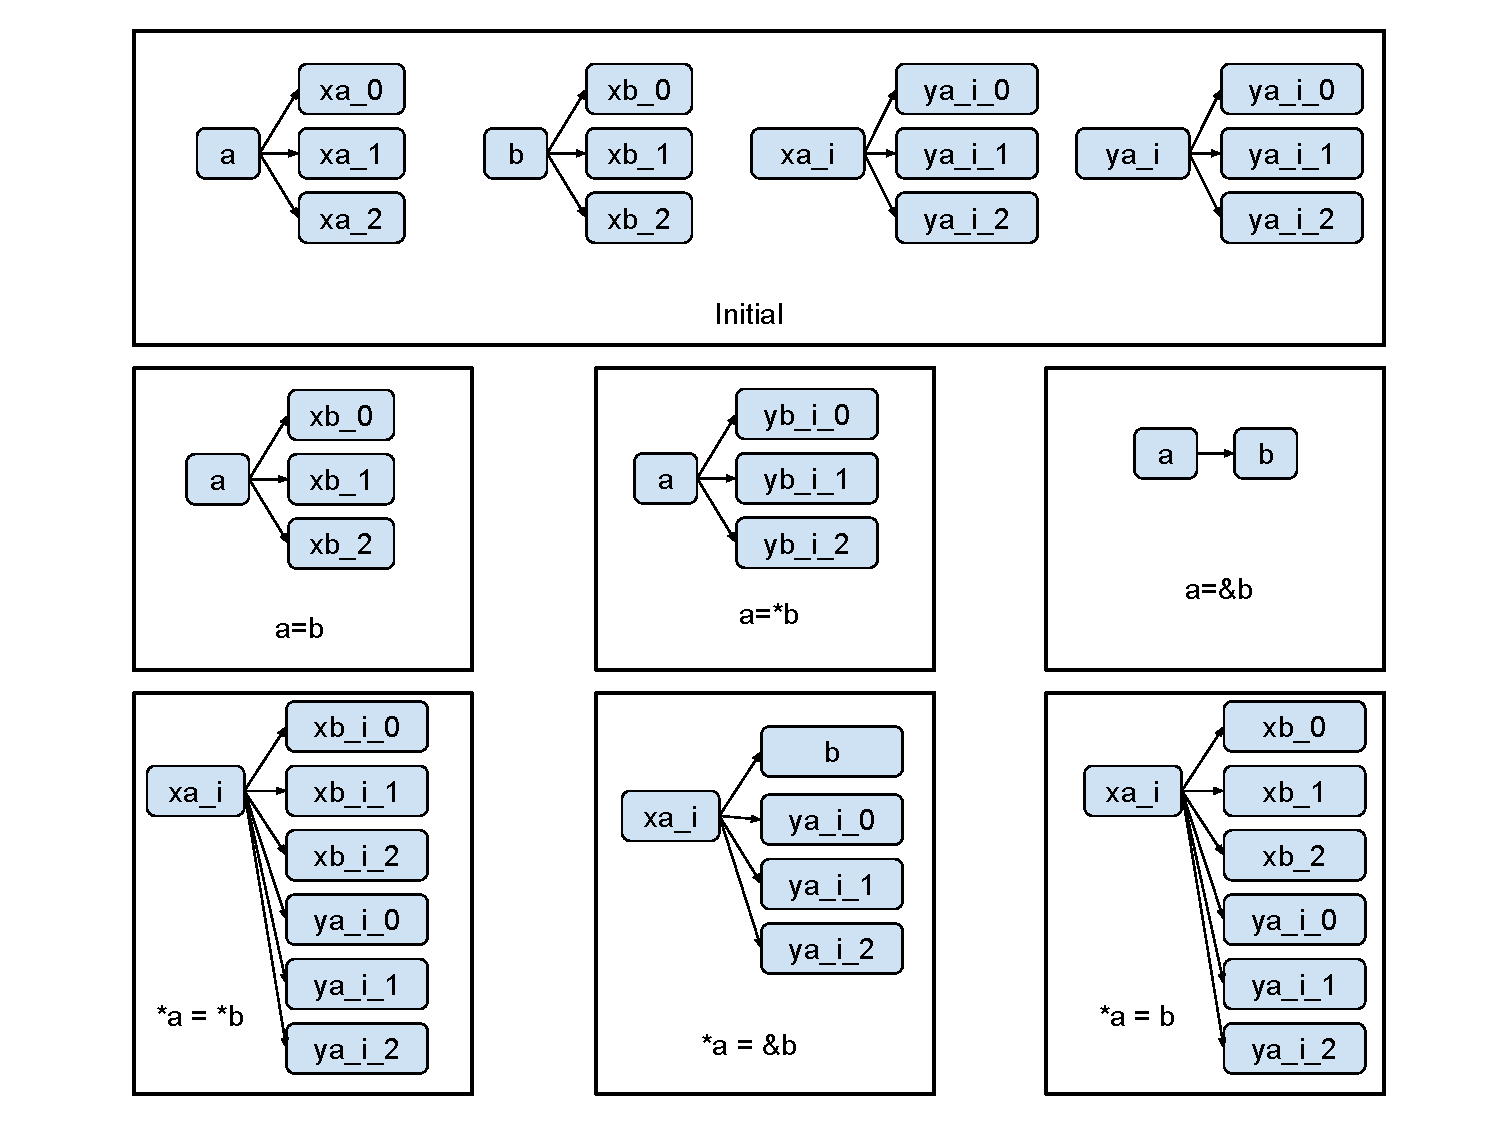
\includegraphics[scale=0.35]{alias/pts-update.pdf}
	\caption{Points-to Updates}
	\label{fig:pts-update}
\end{figure}

Figure~\ref{fig:pts-update} shows the transfer function rules for each
statement type.
%This is illustrated in Figure \ref{fig:pts-update}.
The ``Initial'' section shows a sample initial configuration a points-to relation might have.
Each other region is labeled by a statement, and shows what would change about the points-to relation.
Each time an ``i'' is used on the left, assume that portion is present 3 times, with i ranging from 0 to 2.

For updates to stack slots or registers, we can perform a ``destructive'' update.
This is demonstrated in the \texttt{a =} examples in Figure \ref{fig:pts-update}.
This means that since we know the new value
is the only value the variable could have, we can \emph{replace} the
points-to set.  In the case of pointer write though, we cannot do
this, because our analysis is not field sensitive.

In a field sensitive analysis, this destructive update logic would be
extended to writes through pointers with a points-to size of one,
allowing for more destructive updates and increasing the precision of
our analysis.
We will explain and add field sensitivity shortly in section \ref{sec:field}, but until then, pointer updates need to remain non-destructive.

After we complete the updates to the points-to structure, we remove
all variables which are no longer live according to the previously computed information.
These variables will never be used, so tracking them is imprecise and expensive.

Finally, we perform a mark-and-sweep garbage collection of the tracked pointers, using stack slots, registers, and anything that was pointed to at the entrance of the function as roots.
This last caveat is necessary so that if an argument to a function is written to, and then never used again, the parent will still see the update even though the callee no longer knows how to reference the region.
This allows us to \emph{forget} about allocations which are no longer accessible.

\paragraph{Dataflow}
\begin{lstlisting}[float=*t, caption={Flow Sensitive Pointer Analysis Rules}, label=lst:flowrules]
flow_in(Location, PointsTo^pt_union)
flow_out(Location, PointsTo)

flow_init: flow_in(loc, {}) <- malloc_call {loc}

flow_step: flow_in(dst, pts) <-
  succ {src, dst, is_call: false, is_ret: false} & flow_out(src, pts)

flow_xfer: flow_out(loc, pts2) <-
  flow_in(loc, pts) & updates(loc, us) & kill(loc, ks) & live {loc, live}
  & flow::xfer(pts, us, ks, pts2)
\end{lstlisting}
\begin{lstlisting}[float=t, caption={Process Update}, label=lst:process]
match update {
  (*\bfseries *a = \&b*) =>
    for a_target in pts[a] {
      pts_out.add(a_target, b)
    }
   (*\bfseries a = \&b*) =>
     pts_out.replace(a, {b})
   (*\bfseries a =  b*) =>
     pts_out.replace(a, pts[b])
   (*\bfseries a = *b*) =>
     pts_out.replace(pts[pts[b]])
  (*\bfseries *a =  b*) =>
    for a_target in pts[a] {
      pts_out.add(a_target, pts[b])
    }
  (*\bfseries *a = *b*) =>
    for a_target in pts[a] {
      pts_out.add(a_target,
                  pts[pts[b]])
    }
}
\end{lstlisting}

The overall flow rules we use are shown in  Listing \ref{lst:flowrules}.
Andersen-style analysis formulates updates as inclusion constraints, rather than equality constraints like Steensgaard.
In the initial declaration of predicates, \texttt{flow\_in} is declared to aggregate via set union on each points-to set.
Since each \texttt{flow\_in} value at a location produces a unique \texttt{flow\_out} value, aggregation is not necessary on that predicate.
We create an empty input map at every allocation site, because allocation is the only action which will add information to an empty points-to relation.
\texttt{flow\_step} propagates points-to relations along normal succession edges.
Finally, \texttt{flow\_xfer} performs the meat of the operation, absorbing the update summaries into the current context by applying the transfer function.

\subsection{Inter-procedural Dataflow}
\label{sec:interproc}
Our approach to inter-procedural dataflow follows the example of Reps~\cite{interproc-dataflow} with some modifications.
While many optimizations described there are inapplicable to our domain, the general structure still applies.
At the site of a call, an inter-procedural edge is added from the call site to the target function.
Following this edge elides stack slots which are not currently pointed to.
This is a departure from Reps in that their restricted domain, all local variables were not passed through.
An intra-procedural edge is added which skips over the call, applying effects (see \S \ref{sec:effects}) and clobbering variables not preserved by the function.
Finally, at each return site, an inter-procedural edge which forgets the stack slots local to that function if not pointed to is added.
We do not report an error even if a local stack slot is pointed to, as this is a legal possibility in the case of a recursive call which passes one of its stack variables by reference.
Again, we depart from Reps here by keeping around what would normally be local variables if they are pointed to.

\texttt{flow\_call} and \texttt{flow\_ret} apply when functions are entered and exited to cut down on unnecessary information being propagated around, applying the restrictions for our inter-procedural edges, as described earlier.

\texttt{flow\_call\_over} propagates information at a call site \emph{over} a function call, skipping it but removing definitions for variables known to be overwritten by the function.
This corresponds to the special intra-procedural edge added to our dataflow when processing a call.
This rule also enables analysis through functions which were not provided, albeit with the assumption that the function was effectively a no-op.

\begin{lstlisting}[float=*t, caption={Inter-procedural Rules}, label=lst:interrules]
flow_call: flow_in(dst, pts2) <-
  succ {src, dst, is_call: true} & flow_out(src, pts)
  & flow::call(pts, dst, pts2)
flow_ret: flow_in(dst, pts2) <-
  succ {src, dst, is_ret: true} & flow_out(src, pts) & func {base, contains: dst}
  & flow::ret(pts, base, pts2)
flow_call_over: flow_in(dst, pts2) <-
  call_over {src, func, dst} & flow_out(src, pts)
  & flow::over(pts, pts2)
\end{lstlisting}

\begin{lstlisting}[language=C, float=t, caption={Example (C)}, label=lst:example-c]
char* g() {
	return malloc(1);
}
void f() {
	char* x = malloc(1);
	*x = 'a'; // Safe
	char* g_a = g();
	*g_a = 'a'; // Safe
	char* g_b = g();
	*g_b = 'a'; // Safe
	free(x);
	free(g_a);
	*x = 'b'; // UaF
	*g_b = 'b'; // Safe, but needs context
}
\end{lstlisting}

\subsection{Inter-procedural Flow-Sensitive Example}
In this section, we provide an example of the context- and flow-
sensitive analysis on a simple example shown in
Listing~\ref{lst:example-c}. To provide clarity on how updating alias
sets work, this example does not show data-flow merges, which is a set
union operation as previously described.

Listing \ref{lst:example-c} contains one real use-after-free bug.  We
also show one location that is safe, but without context-sensitivity
an additional false positive will be raised. Without
context-sensitivity, both the allocations for \texttt{g\_a} and
\texttt{g\_b} get merged, making the analysis believe they are aliased
when they are not.

\lstdefinestyle{hilight-asm}{
    language={[x86masm]Assembler},
    moredelim=[is][\color{green}]{|+}{|},
    moredelim=[is][\color{blue}]{|!}{|},
    moredelim=[is][]{|~}{|},
    basicstyle=\footnotesize 
}

\lstinputlisting[style=hilight-asm,
caption={Annotated Flow-Insensitive Analysis},
label=lst:example-asm]{alias/example-annotated.asm}

The corresponding assembly, annotated with comments on the location of
the UaF and alias sets, is shown in Listing~\ref{lst:example-asm}.
Portions of the alias set hilighted in green are new bindings.
Portions in blue are bindings which have been destructively updated.
In the example, the variables are:
\begin{itemize}
	\item The stack slots of f (g has none): sp+24@f, sp+16@f, sp+8@f
	\item All used registers (other than the stack): RDI, RAX
	\item Allocations split on sensitivity, using the form dyn@addr\{stack\}
          \begin{itemize}
          \item Context-insensitive: dyn@5 and dyn@13
          \item Context-sensitive: dyn@5\{19\}, dyn@5\{25\}, dyn@13\{\}
          \end{itemize}
\end{itemize}

The alias sets are annotated as comments. For example, right before
the free on line 35, the alias set is:

\begin{figure}[h!]
\texttt{\{ RAX -> dyn@0; sp+24@f -> dyn@1;
    sp+16@f -> dyn@0; sp+8@f -> dyn@0;
    RDI -> dyn@0 \}}
\end{figure}

This shows that \texttt{RDI} is pointing to the memory location \texttt{dyn@1}, the allocation site for \texttt{x} in the source code.
Right after the \texttt{free} on line 35, the alias set changes to show \texttt{dyn@1} is now free.
The UAF detector would say any pointer that resolves to \texttt{dyn@1} is therefore a use-after-free bug, which happens on
line 53.

If we had been context-sensitive, the points-to relation at 59, the false positive, would instead be
\begin{figure}[h!]
\texttt{\{ RAX -> dyn@5\{25\}; sp+24@f -> dyn@13\{\};
    sp+16@f -> dyn@5\{19\}; sp+8@f -> dyn@5\{25\};
    RDI -> dyn@5\{19\}; dyn@13\{\} -> free@35;
    dyn@5\{19\} -> free@43 \}}
\end{figure}

The key difference here is that \texttt{RAX} points to \texttt{dyn@5\{25\}} rather than just \texttt{dyn@5}, so we can distinguish it from the freed allocation.
This allows context sensitivity to weed out more false positives.




\subsection{Adding Context Sensitivity}
Context-sensitivity requires we only change our \texttt{Location}
values to contain information about the stack.
We add an empty stack to entry points to initialize the new stack-enhanced CFG.
Called functions must copy their control flow graphs to separate versions for every stack at which they are being called.
When generating the target of a call function, we now add the current instruction's fallthrough to the stack as a return address.
If the return address is already on the stack, we truncate the stack so that it is the topmost.

Unfortunately, with an unbounded stack, of our real-world samples (\S \ref{alias:sec:eval:real}), this approach exhausts available resources (128G RAM) for all but \texttt{gnome-nettool}.
To remedy this, we use a $k$-stack approach combined with the stack truncation above.
If a call is made from a location parameterized by a stack, it is first checked to see if the call site is present.
If so, it is truncated as before.
Otherwise, it is pushed onto the stack, and if the stack is longer than $k$, the oldest entry is removed.
In the case of our example, a stack size of 1 would be sufficient, and we'd see the allocations \texttt{dyn@0\{10\}}, \texttt{dyn@0\{11\}}, and \texttt{dyn@1\{\}}.

\subsection{Adding Field Sensitivity}
\label{sec:field}
%TODO add arith and widening
Up until now, we've been treating each memory region like a single homogeneous bag:
Anything written into it ever can be read out again on any subsequent read.
This reduces precision.

In traditional alias analysis, field sensitivity can be done by simply treating each variable with a struct type as though it were several - one for each field.
Unfortunately, in the binary case, things are slightly messier for two reasons: overlapping fields, and variable offset writes.
Since this is only a pointer analysis, not a general value analysis, we only consider fields with size equal to the pointer size.

Previously, we used a simple set to denote what a variable might point to.
We now replace this with a ``field map''.
We will use the word ``reference'' to describe the pair of a variable and an offset.
The offset may be a fixed value, or a special value indicating a computed offset.

A field map has two components: a set of references for unknown offsets, and a set of references for some subset of possible fixed offsets.
If a fixed offset read is performed, we return the offset's set if defined, otherwise the unknown set.
If a computed offset read is performed, we return the union of every set (both unknown and fixed) present in the map.

We split update rules into cases for a single pointer write (so we know which memory cell was updated precisely) and for multiple.

\subheading{Single Pointer}
If a fixed offset write is performed on a variable, we destructively update the set corresponding to that offset.
If a computed offset write is performed, we extend both the unknown set, and every tracked offset to contain the new reference.
If an overlapping field is written to, the field it overlaps is emptied.

\subheading{Multiple Pointers}
If a fixed offset write is performed on a variable, extend the set corresponding to that offset.
If a computed offset write is performed, we extend both the unknown set, and every tracked offset to contain the new reference.
If an overlapping field is written to, nothing happens.

This structure is conservative so long as we accept the assumption that pointers are not constructed piece-wise.
Specifically, if pointers are constructed over the course of multiple writes, we will not know about them.
This limitation was present in the previous, field insensitive formulation, but becomes more obvious in the description of the field sensitive extension.
This practice is extremely uncommon (outside bulk copy functions like \texttt{memcpy}, which may be summarized), so we accept this limitation to limit the need to reason about the exact possible values of a computed offset.

Unfortunately, this formulation gives the alias analyzer slightly too much power.
Specifically, it can now count.
Despite the fact that we did not model actually performing arithmetic, a pointer being incremented in a loop will look like repeatedly examining relative offsets of a struct.
To deal with this, we add a widening operator\footnote{
	A widening operator is an addition to a dataflow analysis which provides termination by moving further on the lattice than is strictly necessary under certain conditions.
}which, if the same variable points to a fixed limit or more offsets in a region, will replace it with pointing to an unknown offset to that region.
This reclaims termination.

\subsection{Recent Allocation Domain}
\label{sec:effects}
Using the site or site and size of an allocation to define the allocation domain is fairly common.
However, this can have poor behavior around loops:

\begin{lstlisting}
char* x;
while(1) {
site_0:
	x = malloc(1);
	*x = 'a';
	free(x);
}
\end{lstlisting}

If running a dataflow computation to fixpoint, on the second
iteration, the allocation for \texttt{site\_0} will appear already
freed.  The usual response to this type of imprecision is to unroll
loops a fixed number of times.  However, our tool is intended to be
complete (assuming a complete control flow graph, provided functions,
etc.) so we want to avoid fixed unrollings.

To this end, we extend our allocation domain with a ``recent'' bit, similar to the MRAB vs NMRAB abstraction~\cite{vsa}, though for different purposes.
Relative to a concrete trace, the address most recently given by an allocation at a given site belongs to the set where ``recent'' is true.
All other addresses issued by that site belong to the set where ``recent'' is false.
In our static form, a value belongs to the recent set for an allocation site if there exists some trace for which it was the last allocated from that site.
It belongs to the non-recent set if there exists some trace for which it was not most recently allocated.
Note that once in static form, the recent set may have more than one member, and may even intersect with the non-recent set.

This extension is a departure from the normal Andersen alias analysis.
It is only for precision, not correctness.
It can essentially be viewed as 1 bit path-sensitivity, where path-sensitivity would be parameterizing on entire sequences of instructions which could be taken to reach the current point.

To implement this in our static alias analysis, we construct summaries for each function of allocations and possible allocations.
When processing the edge which skips the function which is meant to propagate variables not accessible to it, we update the points-to relation using information from this summary to keep recency information accurate.
We do this by modifying the behavior of \texttt{flow\_call\_over} to update the caller points-to to represent what may have happened in the callee.

We define an ``effect'' to be a set of definite allocation sites and a set of possible allocation sites that occur when a call is made.
To apply an effect to a points-to set:
For every definite allocation site, make the recent bit false.
For every possible allocation site, duplicate any recent references to have both recent and non-recent values.
Listing~\ref{lst:recent} shows this change.

%To this end, we amend the rules as in Listing \ref{lst:recent}
\begin{lstlisting}[float=*t, caption={Rules for Recent Domain}, label=lst:recent]
flow_call_over: flow_in(dst, pts2) <-
  call_over {src, func, dst} &
  flow_out(src, pts) &
  (*\bfseries func\_effect \{func, effect\} \&*)
  (*\bfseries flow::over\_effect(pts, effect, pts2)*)

local_effect {base: Location, local: Location, effect: Effect}
func_effect {func: Location, effect: Effect^effect_merge}

effect_init: local_effect {base, local: base, effect: no_op} <- func {base}
effect_ret: local_ret: func_effect(base, effect) <-
  succ {src: local, is_ret: true} &
  local_effect {base, local, effect}
effect_xfer: local_effect {base, local: local2, effect} <-
  succ {src: local, dst: local2, is_call: false, is_ret: false} &
  local_effect {base, local, effect}
effect_call: local_effect {base, local: local2, effect: effect2} <-
  call_over {src: local, func: remote, dst: local2} &
  func_effect {func: remote, effect: effect_call} &
  local_effect {base, local, effect} &
  effect::sequence_effect(effect, effect_call, effect2)
effect_malloc: local_effect {base, local: local2, effect: effect2} <-
  succ_over {src: local, dst: local2} &
  local_effect {base, local, effect} &
  malloc_call {loc: local} &
  effect::malloc(effect, local, effect2)
\end{lstlisting}

There are four new functions here.
\texttt{effect\_merge} will merge two local effects at a confluence point.
It does this by intersecting their definite allocations, and migrating all other allocations to possible allocations.
\texttt{flow::over\_effect} will apply the effect to the points-to set in addition to its earlier responsibilities.
\texttt{effect::sequence\_effect} will update the currently processed effect with the called function's effect by unioning together both possible and definite effects, then removing those possible effects which are also definite.
\texttt{effect::malloc} just adds the current site as a definite allocation to the effect.

The result is that these effect summaries allow greater precision over allocation sites, similar to what is achieved through loop unrolling, but without sacrificing fix-point semantics.

In our example earlier, this would give rise to three allocations - \texttt{dyn@0}, \texttt{dyn@1+old}, and \texttt{dyn@1}.
This would suppress the false positive by distinguishing between the two invocations of \texttt{g}.
However, were a third added, it would not be able to distinguish between the first two invocations of \texttt{g}.

\subsection{Use-after-Free}
With alias relationship in hand, we must determine which reads and writes in the program are use-after-free candidates.
For the flow and flow \& context analyses, we can augment the alias analysis itself to track most of this information for us.
When a free occurs, we generate a special form of the \texttt{*a = \&b} summary, with \texttt{a} as the pointer being freed, and \texttt{b} as a special value representing things freed at that location.
This is as presented in Listing \ref{lst:uafflow}.
\texttt{read\_vars} generates pointer access information from actual assembly instructions, and \texttt{use\_vars} imports it from summaries which can do things like determine argument count to \texttt{printf}.

\begin{lstlisting}[label=lst:uafflow, caption={Tracking Frees with Flow Sensitivity}]
read_vars: deref_var(v, loc) <-
  lift {loc, bil} &
  func {base, contains: loc} &
  uaf::reads_vars(bil, v)
use_vars: deref_var(v, loc) <-
  uses(r, loc) &
  uaf::use_vars(r, v)

free_summary: summary(loc, s) <-
  free_call{loc, args} &
  uaf::free_summary(args, s)
uaf_flow: uaf_flow(v, loc, loc2) <-
  deref_var(v, loc2) &
  flow_in(loc2, pts) &
  flow::is_freed(pts, v, loc)
\end{lstlisting}

However, this approach only works with alias information that is at least flow sensitive.
Without flow sensitivity, any pointer which was ever freed will appear freed everywhere in the program, even before it was freed.
As a result, the false positive rate would be absurd, and such a detector would be more a heap-access detector than a use after free detector.
To help it along and make the difference in false positive rates more about the precision of the alias information rather than the ability to track state changes, we add a few extra conditions to report a use after free without flow sensitivity by essentially doing flow sensitive tracking of the freed-property only.

\begin{lstlisting}[label=lst:uafins, caption={Tracking Frees Insensitively}]
base_freed: freed_base(v, loc) <-
  free_call {loc, args} &
  uaf::free_args(args, v)
all_freed: freed_var(v2, loc) <-
  freed_base(v, loc) &
  steens_point(v, vs) &
  uaf::expand_vars(vs, v2)

path_init: path_exists(loc, loc) <-
  freed_base(_, loc)
path_step: path_exists(loc, loc3) <-
  path_exists(loc, loc2) &
  succ_any {src: loc2, dst: loc3}

uaf: uaf(v, loc, loc2) <- freed_var(v, loc) & path_exists(loc, loc2) & deref_var(v, loc2)
\end{lstlisting}

The implementation of this modification is shown in Listing \ref{lst:uafins}.
In the first stanza, we mark the variable freed by the free call and everything it aliases with as potentially freed at that location.
In the next, we find those parts of the program reachable from the free site.
We then finalize the results by saying that if a path exists from a freed variable to a dereference of that same variable, then there is a use after free candidate.
While this is certainly imperfect, going much further would begin to graft flow sensitive information into the otherwise insensitive analysis.

\section{Implementation}
\label{alias:sec:impl}
Our implementation consists of 3k lines of Rust and 234 lines of datalog.
Each additional sensitivity (field, context, flow, recency) is implemented by adding an additional datlaog file.
The switches to determine which sensitivities actually run operate by adding initial facts to the database to suppress unwanted rule triggers.
As a result of this design, other than field sensitivity (which requires significant logic in both the constraint generator and points-to set structures), these additional sensitivites can be compiled out safely by simply removing the rules in question (and their associated bound functions).

\subsection{Limitations}
Our system is conservative in almost all cases, but there are a few notable exceptions.
If the provided file is linked against files which are not provided, their functions will be assumed to effectively be no-ops.
If in reality, these functions free memory or write to the heap, this may cause missed vulnerabilities.
The system uses the BAP control flow graph and any indirect jump resolution and the analysis assumes they go nowhere; we do no additional resolution beyond \texttt{ret} calls.
%This may result in an incomplete control flow graph, which in turn can lead to %missed bugs.
Control flow recovery is a general problem in binary analysis and not specific to our approach.
Essentially, if a prerequisite step gives our algorithm incomplete information, it will produce an incomplete result.
This was sufficient for the programs analyzed, which are written largely in C, but some resolution would be required to achieve good quality result on C++ programs which use vtables or programs which use a callback architecture (and so rely heavily on function pointers).

We assume the transfer of a pointer from one place to another will take place in a single assembly instruction - we do not model ``the first 3 bytes of a pointer to x'' for example.
Finally, we assume that a traditional stack discipline is being followed for purposes of points-to minimization in the sensitive cases.
If it is not, aliases from stack calculations pointing above or below your own stack frame may be missed.

\section{Evaluation}
\label{alias:sec:eval}
Our evaluation has 3 major components.
\begin{itemize}
\item Juliet - How do we perform on a labeled (true positives, false positives, false negatives) data set?
\item Real World Bugs - Can we detect real bugs? 
\item Ubuntu \texttt{\$PATH} - How often do we alarm on real bug-free code?
\end{itemize}

We evaluate over the Juliet test set both for comparability with other work~\cite{tac, juliet-eval-static-source} and to act as a baseline for our detection power and false positive rates.
It helps answer the question ``In the absences of confounding factors from the real world, how well does this work?''.
We also evaluate over real use-after-free bugs pulled from MITRE's CVE database.
Evaluating on these verifies that real world code, while potentially confounding, does not stop our technique from functioning altogether.
It also provides a measurement of the false positive rate in the presence of true positives.
Finally, we evaluate over a variety of believed-good binaries.
The intent behind this evaluation is to get a better idea of false positive rates and analysis costs for average programs believed to be non-buggy.

\subsection{Juliet}
IARPA released the Juliet test suite~\cite{juliet} as a way of providing standardized examples of CWEs.
By building only those corresponding to use-after-free, we get a high density test suite.

All three sensitivities find all intended bugs in Juliet.
Insensitive analysis generates 39834 false positives, reducing to 0 with flow sensitivity.
Run time was 19m30s for the flow sensitive version, and 30m4s for insensitive.
However, the insensitive variety generates its alias information as of 3m23s.
The system spent the remainder of the time generating reachability information.

Unfortunately, while Juliet serves as a good test for true positives, it does not do much to elicit false positives from our system, which is why both our performance and others' look too-good-to-be-true here.
Within the negative tests, there is little in the way of things that checkers are traditionally weak against (data structures, recursion, loops, etc.).
For this reason, it is important to evaluate ourselves on real world code as well.

\subsection{Live CVEs}
\label{alias:sec:eval:real}
Our system successfully detects 7 real bugs across 6 programs.
All sensitivities of the checker detected all bugs.
We assume that all potential use after frees which do not match the known bugs in each of these programs are false positives.

\begin{figure*}
\begin{center}
\begin{tabular}{|c|c||c|c|c|c|}
\hline
Program & Sensitivity & Run time & Memory & False Positives & Binary Size\\
\hline \hline
\multirow{3}{*}{gnome-nettool} & Insensitive & 38s & 1G & 1851 & \multirow{3}{*}{156k}\\
	& Flow & 30s & 1G & 0 &\\
	& Flow + Ctx & 2m34s & 2G & 0 &\\
	\hline
\multirow{3}{*}{goaccess} & Insensitive & 4m35s & 15G & 387459 & \multirow{3}{*}{635k}\\
	& Flow & 16m14s & 10G & 112420 &\\
	& Flow + Ctx & 43m34s & 34G & 87 &\\
	\hline
\multirow{3}{*}{libarchive} & Insensitive & 1m23s & 3G & 4917 & \multirow{3}{*}{366k}\\
	& Flow & 34s & 1G & 852 &\\
	& Flow + Ctx & 22m12s & 44G & 7 &\\
	\hline
\multirow{3}{*}{shadowsocks-libev} & Insensitive & 2m12s & 5G & 130760 & \multirow{3}{*}{631k}\\
	& Flow & 3hr46m21s & 62G & 22357 &\\
	& Flow + Ctx & 3hr53m26s & 72G & 115 &\\
	\hline
\multirow{3}{*}{mdadm} & Insensitive & 16m45s & 31G & 1056570 & \multirow{3}{*}{768k}\\
	& Flow & 2hr24m13s & 42G & 270683 &\\
	& Flow + Ctx & 12hr10m43s & 111G & 14566 &\\
	\hline
\multirow{3}{*}{isisd} & Insensitive & 3m46s & 8G & 58241 & \multirow{3}{*}{451k}\\
	& Flow & 18m49s & 9G & 11776 &\\
	& Flow + Ctx & 22m32s & 25G & 513 &\\
	\hline
\end{tabular}
\end{center}
\caption{Real CVE Performance}
\label{fig:cveperf}
\end{figure*}

\begin{figure*}
	\begin{center}
	\begin{tabular}{|c||c|c|c||c|c|c||c|c|}
		\hline
		Sensitivity & \multicolumn{3}{c||}{Run time} & \multicolumn{3}{c||}{Memory} & \multicolumn{2}{c|}{Alarms} \\
		\hline
		& Avg & Median & Stdev & Avg & Median & Stdev  &Avg & Imp\\
		\hline\hline
		Insensitive  & 2m26.1s & 58.4s & 3m38.1s & 241.7M & 34.1M & 1.9G & 73.1 &\\ \hline
		Flow & 2m14.2s & 54.7s & 3m19.6s & 236.8M & 34.1M & 1.9G & 0.5 & 93.1\% \\ \hline
		Flow and Ctx  & 2m22.1s & 55.6s & 3m54.9s & 349.2M & 34.0M & 2.3G & 0.2 & 43.5\% \\ \hline
	\end{tabular}
	\end{center}
	\caption{Ubuntu \texttt{/usr/bin} Performance}
	\label{fig:ubperf}
\end{figure*}

Note that while the insensitive analysis completes quickly and cheaply for every binary, the false positive rates are so high that the output would be difficult to use.
Flow sensitivity reduces false positives significantly.
Manual analysis reveals that most remaining false positives are either due to data structure usage (which decreases the precision of the alias analysis), confused allocation sites from wrapped malloc constructors, and infeasible paths.
Context sensitivity gives additional improvements by helping to differentiate between instances of calling wrapped mallocs (e.g. \texttt{new\_foo()} to allocate and initialize a \texttt{foo}).


Performance for insensitive and flow-sensitive analyses appears similar in large part because the generation of a global program reachability graph for each \texttt{free} is costly.
If the analysis is instead timed in phases, the alias-analysis-only portion for the insensitive system takes seconds, while it takes the bulk of the non-CFG-recovery time in a flow-sensitive analysis.

For the known-vulnerable set, flow sensitivity reduced the false positive set by an average of 90\%, and context sensitivity reduced it by an additional 84.1\%.
The false positive reduction for the addition of flow sensitivity is immense, and the increase in time and space needed for the alias analysis was manageable for programs in our known-vulnerable set, the largest of which was 768kb.
Adding context sensitivity further increased the time and space cost, but still yielded a major increase in precision.

\subsubsection{GUEB}
The author of the GUEB~\cite{gueb} tool made his tool open source\footnote{
	\url{https://github.com/montyly/gueb}
}, allowing us to compare against it.
We connected IDA, BinNavi, and GUEB and ran the system over the same bugs we evaluated against.
As a caveat, we could not feed them the same binaries our tool consumed - their tool's stack only accepts 32-bit, so we recompiled the same vulnerable programs in 32-bit mode.

Figure~\ref{fig:guebperf} shows the performance.
The crashes derive from unhandled cases in the input, and not fundamental to their methods.
The undetected bugs occur due to their choice to not follow back edges (either as recursion or loops) when computing their VSA.
This is an understandable choice, since VSA can become slow and be difficult to force convergence for when cycles are present in the input, but in this case it caused their analysis to miss bugs.
Likely due to this forwards-only approach, GUEB terminated rather quickly on all inputs.

In Listing~\ref{lst:isisd-gueb}, we can see one of the real vulnerabilities the lack of a fixpoint fails to detect.
The loop knows that \texttt{adj} is allocated and non-null on entry, so the first time through the loop is always fine.
However, some paths through the loop free \texttt{adj}, and go around the loop again.
At this point, a use-after-free can occur.
If back edges are not followed, the analysis cannot detect this.

\begin{figure}
\begin{center}
\begin{tabular}{|c||c|c|}
\hline
Program & False Positives & Bug Found? \\
\hline \hline
	gnome-nettool & 2 & Yes\\
	goaccess & crash & crash\\
	libarchive & 222 & Yes\\
	shadowsocks-libev & crash & crash\\
	mdadm & crash & crash\\
	isisd & 596 & No\\
\hline
\end{tabular}
\end{center}
\caption{GUEB Performance}
\label{fig:guebperf}
\end{figure}

\begin{lstlisting}[language=C, float=t, caption={\texttt{isisd} Vulnerability}, label=lst:isisd-gueb]
// ... (adj is allocated and constructed here)
for (level = IS_LEVEL_1; level <= IS_LEVEL_2; level++) {
	// ...
	else if (new_state == ISIS_ADJ_DOWN) {
		// ...
		isis_delete_adj(adj);
	}
}
// ...
\end{lstlisting}


\subsection{Ubuntu Path Sample}
Now that we know that our program will alert us to real world vulnerabilities, we also want to know how it will behave in the case where no expected vulnerabilities are present.
To this end, we ran our program across \texttt{/usr/bin} on a default Ubuntu Xenial installation, as shown in Figure~\ref{fig:ubperf}.

Adding flow sensitivity provided an average reduction in bug candidates of 93.1\% in those situations where the insensitive code found at least one candidate.
Then adding context sensitivity ($k$ = 1) reduced it by an additional 43.5\%, in those situations where the flow sensitive analysis had a bug candidate, and the context sensitive analysis terminated.

Manual auditing of the reported bugs did not reveal any true bugs, but did show that a common pattern amongst false positives was functions for whom one path freed and replaced a pointer, and the other did neither, and they rejoined.
A more aggressive analysis for dead variables could remedy this by pruning them to allow the freed region to leave the points-to relationship before the paths rejoined.

The system emitted a maximum of 22 reports on individual binaries (and this worst case had most of them clustered in the same code area).
This was few enough reports to enable practical manual auditing by a single individual.
Unfortunately, none of these reports corresponded to real bugs upon examination.
This does not guarantee these programs are bug free - while we have a conservative analysis, that is dependent on seeing the entire control flow graph.
In this case this condition is not met.
Some C++ programs which use vtables are present in this path - calls to member functions there will appear as no-ops.
Function pointers are similarly considered to be no-ops.
Calls into libraries which were not analyzed with the binary are similarly absent.
Finally, some of these are GUI or threaded applications, which utilize a callback system we again do not handle control flow edges for.

\FloatBarrier
\section{Conclusions}
We presented \aliasname, a novel, open source, binary-only use-after-free detector.
In \aliasname, we demonstrated how to adapt alias analysis techniques from source-level analysis to compiled code.
This reduced the reliance of binary analysis on VSA in cases where its full power is not required.
We evaluated three points in the design space of alias analysis for purposes of detecting use-after-free bugs, comparing both the performance cost and precision of different sensitivity combinations, including no sensitivity, flow sensitivity, context sensitivity, and field sensitivity.
Over known-vulnerable programs, flow sensitivity removed 90\% of false positives, with context sensitivity removing an additional 93.1%.
When testing believed safe programs, we observed 93.1\% and 43.5\% reductions respectively.
Use of analyses lighter than VSA allows for whole program analysis of medium-sized programs for use-after free vulnerabilities, with additional computational resources allowing for increased precision.


\bibliographystyle{IEEEtran}
\bibliography{IEEEabrv,marduk}
\end{document}
